\section{Implementation Details}
\label{appendix:method}

Figure~\ref{fig:sparse_computation_diagram} presents a more detailed workflow of \name{}. The left diagram shows how an input $y$ performs the sparse MHA with selected indices ${0, 3}$, predicted by the head predictor. Similarly, the right diagram shows how an input $y$ performs the sparse MLP with selected indices ${0, 2}$, predicted by the neuron predictor of that layer.

\begin{figure}[h]
  \centering
  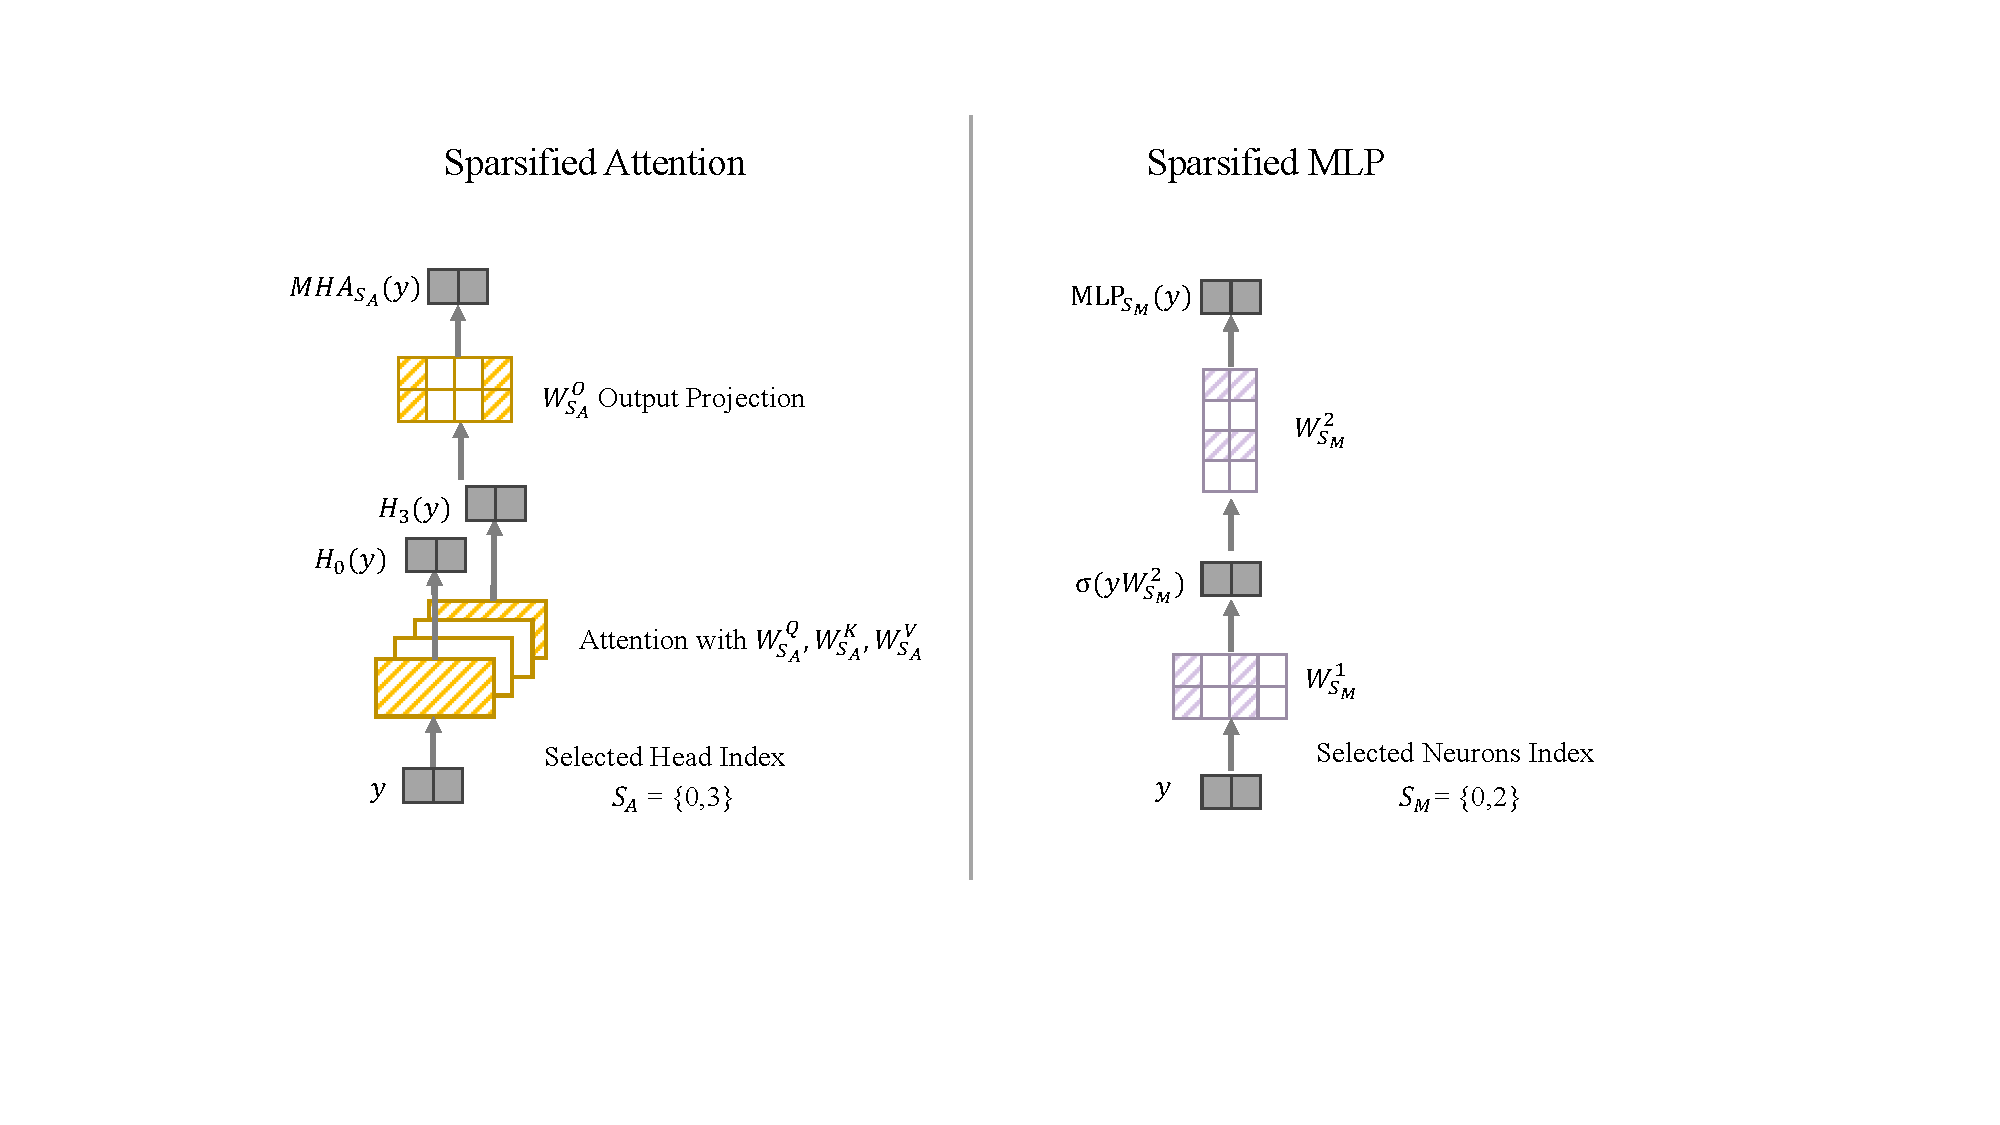
\includegraphics[width=0.8\textwidth]{figure/sparse_computation_diagram.pdf}
  \caption{Detailed diagram on the sparsified computation process of MLP and Attention. Notation refers to Section~\ref{sec:formulation}}
  \label{fig:sparse_computation_diagram}
\end{figure}

Next, we will present a general explanation of two optimizations we used in \name{} implementation. Kernel fusion: A standard implementation of sparse matrix-vector
  multiply (e.g., $Wx$ in PyTorch) that separately indexes a subset of the matrix
  $W[\mathrm{idx}, :]$ before multiplying with input $x$ would incur 3$\times$ the
  amount of memory IOs: one to load a subset of $W$ from GPU memory, one to
  write that subset to a different contiguous region in memory, and one to load
  that (now contiguous) subset in again to multiply with $x$.
  Similarly, to use sparse matrix multiply routines (e.g., cuSparse), we would
  first need to convert $W[\mathrm{idx}, :]$ to sparse format, again incurring
  more memory IOs.
  We instead fuse the indexing and the multiplication step: we load a subset of
  $W[\mathrm{idx}, :]$ to memory, along with $x$, perform the multiply, then
  write down the result.
  This fused implementation (in Triton~\citep{tillet2019triton}) yields up to
  4$\times$ speedup compared to a standard PyTorch implementation (Section~\ref{sec:mlp_attn_benchmarks}). Memory coalescing: the weight matrices are conventionally stored in
  row-major format.
  This allows us to load $W[\mathrm{idx}, :]$ optimally (as the second dimension
  is contiguous in memory).
  However, for cases where we need to load $W[:, \mathrm{idx}]$ (attention
  output projection and the 2nd weight matrix in the MLP) this format
  significantly slows down memory loading, as $\mathrm{idx}$ could contain
  indices pointing to non-contiguous memory.
  A simple solution is to store these matrices in column-major format (i.e.,
  storing $W^\top$ in contiguous row-major format), then use the same fused kernel
  above.
  This transposition is done once when loading the model, and incurs no added
  cost during generation.